\documentclass{standalone}
\usepackage{tikz}
%------------tikz Setup------------

\tikzstyle{ball} = [circle,shading=ball, ball color=black,
    minimum size=1mm,inner sep=1.3pt]
\tikzstyle{miniball} = [circle,shading=ball, ball color=black,
    minimum size=1mm,inner sep=0.5pt]
\tikzstyle{mminiball} = [circle,shading=ball, ball color=black,
    minimum size=0.6mm,inner sep=0.1pt]
\usetikzlibrary{arrows.meta}
\usetikzlibrary{angles, quotes}
\tikzset{>={Latex[length=2mm,width=1.5mm]}}
\tikzset{->-/.style={decoration={markings, mark=at position #1 with
  {\arrow{>}}},postaction={decorate}}}
\usetikzlibrary{decorations.pathmorphing}
\usetikzlibrary{decorations.pathreplacing}
\usetikzlibrary{arrows.meta,calc}
\usetikzlibrary{bending}
\usetikzlibrary{decorations.markings,shapes.geometric}
\tikzset{->-/.style={decoration={markings, mark=at position #1 with
  {\arrow{>}}},postaction={decorate}}}
\tikzset{-|-/.style={decoration={markings, mark=at position #1 with
  {\arrow{stealth}}},postaction={decorate}}}
\tikzset{movearrow/.style 2 args ={
        decoration={markings,
    mark= at position {#1} with {\arrow{#2}} ,
        },
        postaction={decorate}
    }
}


\begin{document}
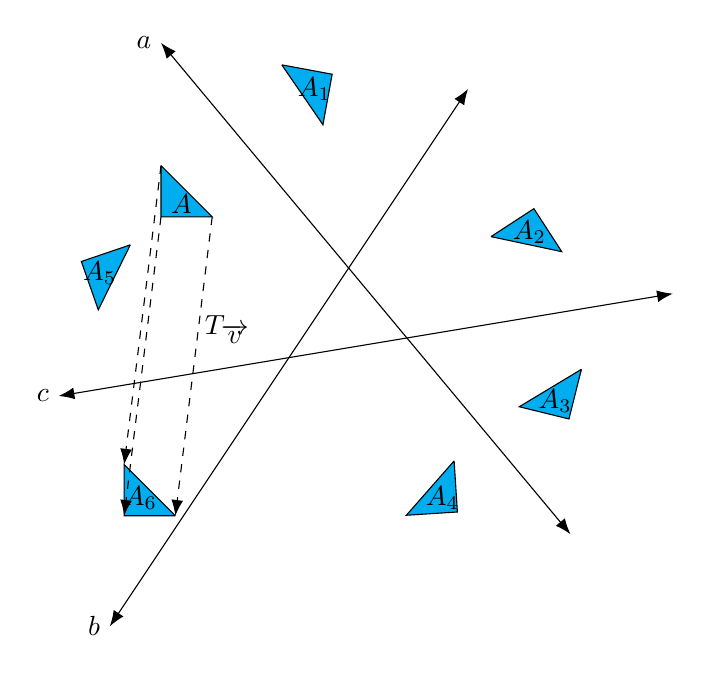
\begin{tikzpicture}
\begin{scope}[scale=0.65]
    %lines
    \draw[<->] (-4,4.4) -- (4,-5.2);
    \draw[<->] (-5,-7) -- (2,3.5);
    \draw[<->] (-6,-2.5) -- (6,-0.5);
    %line labels
    \node[left] (a) at (-4,4.4) {$a$};
    \node[left] (b) at (-5,-7) {$b$};
    \node[left] (c) at (-6,-2.5) {$c$};
    %triangles
    \draw[fill=cyan] (-4,2) -- (-3,1) -- (-4,1) -- (-4, 2);
    \draw[fill=cyan] (-1.64,3.97) -- (-0.836,2.8) -- (-0.656,3.787) -- (-1.64,3.97);
    \draw[fill=cyan] (2.448,0.614) -- (3.286,1.16) -- (3.83,0.32) -- (2.448,0.614);
    \draw[fill=cyan] (4.214,-1.979) -- (3.971,-2.949) -- (3,-2.71) -- (4.214,-1.979);
    \draw[fill=cyan] (1.727,-3.768) -- (1.791,-4.766) -- (0.794,-4.83) -- (1.727,-3.768);
    \draw[fill=cyan] (-4.6,0.453) -- (-5.225,-0.817) -- (-5.556,0.128) -- (-4.6,0.453);
    \draw[fill=cyan] (-3.72,-4.84) -- (-4.72,-3.84) -- (-4.72,-4.84) -- (-3.72,-4.84);
    %triangle labels
    \node(1) at (-3.6, 1.25) {$A$};
    \node(2) at (-1, 3.5) {$A_1$};
    \node(3) at (3.2, 0.7) {$A_2$};
    \node(4) at (3.7, -2.6) {$A_3$};
    \node(5) at (1.5, -4.5) {$A_4$};
    \node(6) at (-5.2, -0.1) {$A_5$};
    \node(7) at (-4.4, -4.5) {$A_6$};
    %vectors
    \draw[->,dashed] (-4,2) -- (-4.72,-3.84);
    \draw[->,dashed] (-3,1) -- (-3.72,-4.84);
    \draw[->,dashed] (-4,1) -- (-4.72,-4.84);
    \node(8) at (-2.7, -1.2) {$T_{\overrightarrow{v}}$};
\end{scope}
\end{tikzpicture}
\end{document}